\chapter{Night 7: PCA and Eigenfaces}

\begin{learningobjectives}
\emph{Concepts}
\bi
\item Understand the connection between PCA and eigenvalues and eigenvectors.
\item Understand how to use PCA to carry out data compression.
\item Understand the idea of using Eigenfaces to do facial recognition.
\ei
\emph{MATLAB skills}
\bi
\item Use ``eig'' to carry out a PCA.
\item Implement facial recognition using PCA.
\item Determine the accuracy of PCA for different numbers of principal components.
\ei
\end{learningobjectives}

\section{Principal Component Analysis Revisited}

As we in class, PCA is an algorithm in which we express our original data along the eigenvectors corresponding to the largest eigenvalues of the covariance matrix.  We examined the property of PCA that it if we project our data onto these vectors, this will lead to maximizing the variance of the projected data.  To refresh your memory further, here is the temperature plot for Boston, Sao Paolo, and Washington DC.

\begin{center}
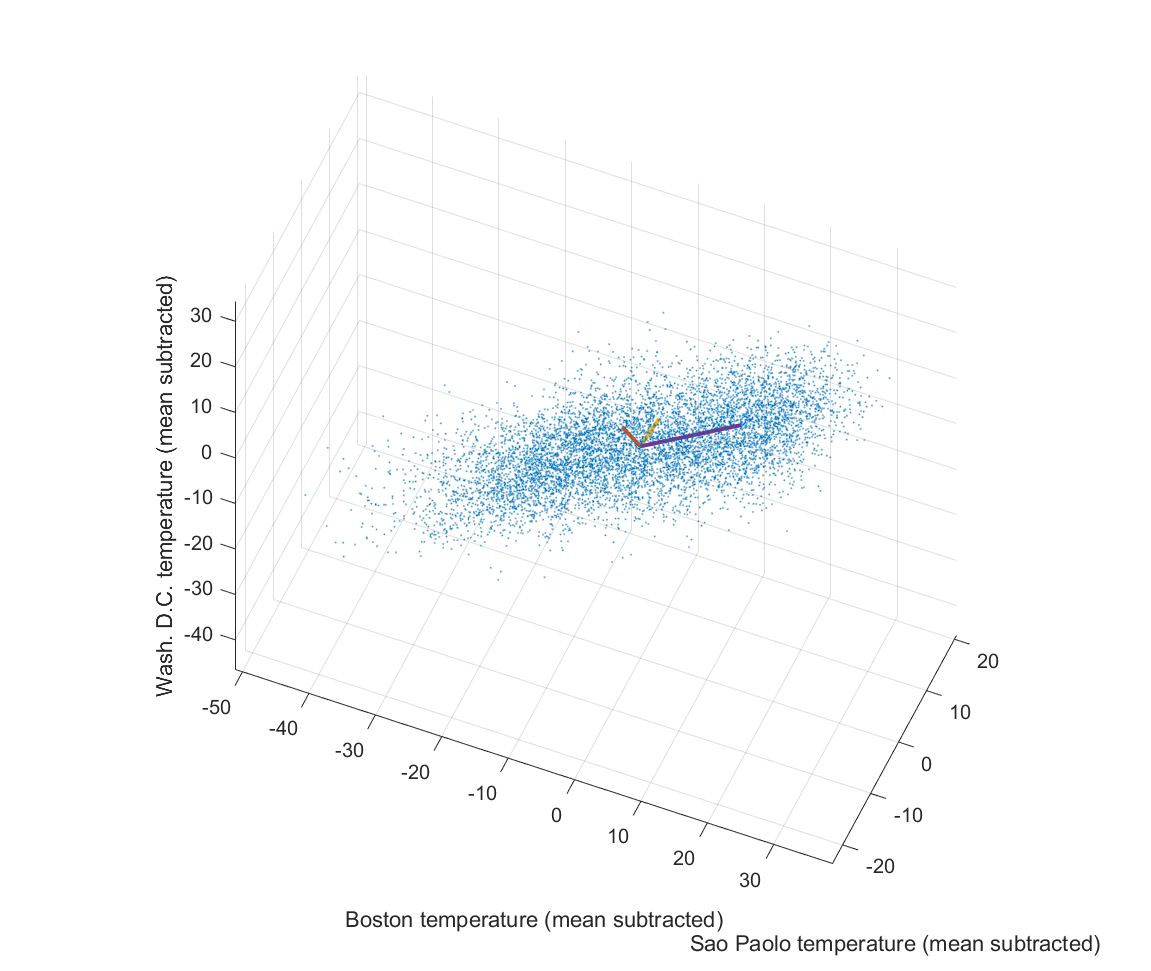
\includegraphics[width=0.5\textwidth]{FacesNight6/figs/tempplot.png}
\captionof{figure}{Temperatures in three cities and the eigenvectors of the covariance matrix.}
\label{temps}
\end{center}

We also briefly mentioned a second property of PCA, which is that it can be thought of as an optimal way to compress our data down to a smaller set of numbers.  This idea, also known as dimensionality reduction, is going to be a view that we explore in this assignment.
%
%\subsection{Eigenvalues and eigenvectors of Covariance Matrices}
%
%First, let's make an observation: \textit{If $\mathbf{R}$ is a covariance matrix, then $\mathbf{R}$ has non-negative eigenvalues and orthogonal eigenvectors.} (The derivations of these properties are presented at the end of this document, but we won't go into it here.) This is important because we want to do PCA on the covariance matrix and we can only do PCA on a matrix whose eigenvectors are orthogonal.
%
%Why do we want to do PCA on the corvariance matrix? Because the eigenvalues and eigenvectors of a covariance matrix tell us something about the spread of the data in different directions. In the Night 6 assignment you produced a plot like the one below, which shows the eigenvectors of the covariance matrix for temperature data in three cities.
%
%\begin{center}
%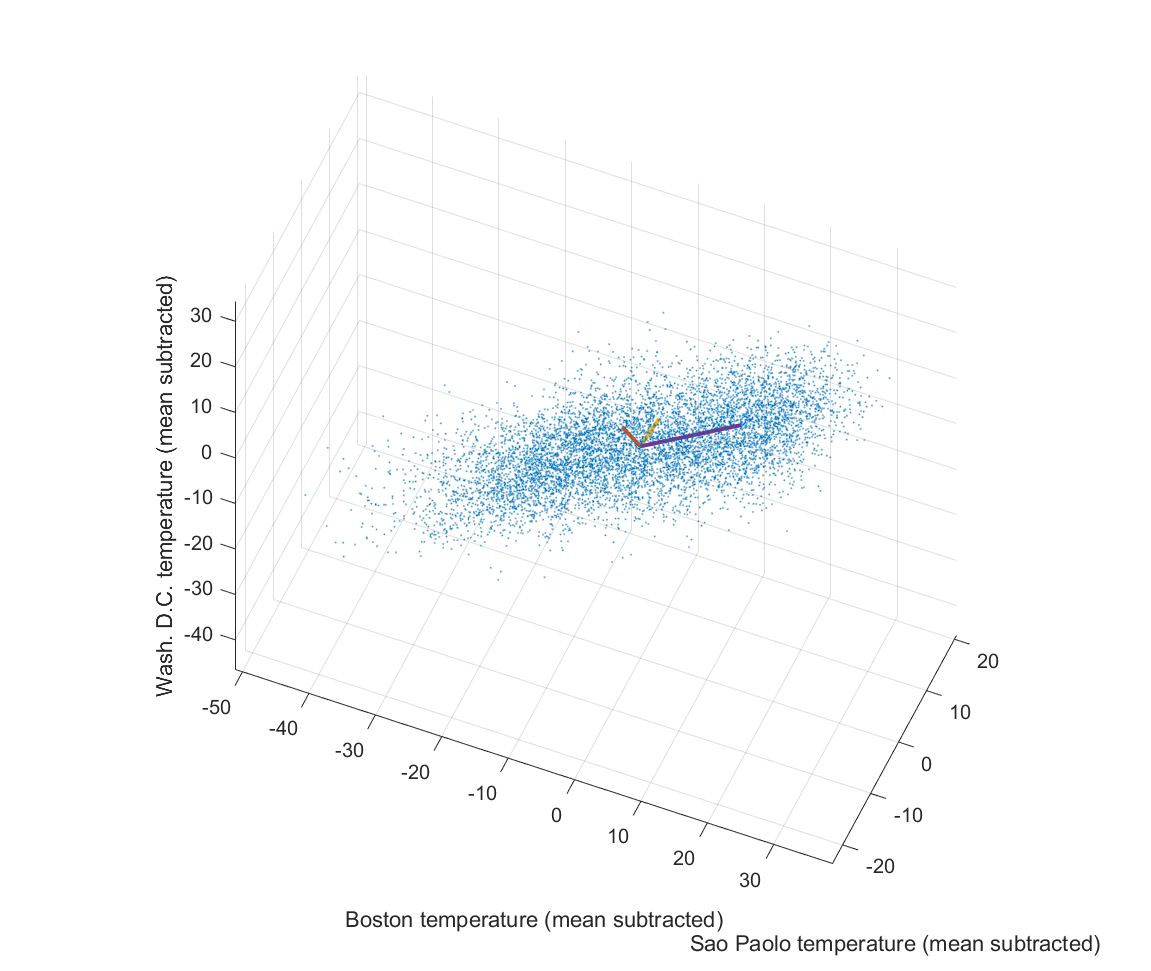
\includegraphics[width=0.7\textwidth]{FacesNight6/figs/tempplot.png}
%\captionof{figure}{Temperatures in three cities and the eigenvectors of the covariance matrix.}
%\label{temps}
%\end{center}
%
%Suppose that the eigenvalues of a covariance matrix corresponding to a given data set are $\lambda_1, \lambda_2, \cdots \lambda_n$, and the corresponding eigenvectors are $\v_1, \v_2, \cdots \v_n$. Assume that $\lambda_1>  \lambda_2 > \cdots > \lambda_n$. As we saw in the temperature data example in Night 6, $\v_1$ points in the direction of greatest variation in the data.  Moreover, of all the directions which are orthogonal to $\v_1$, $\v_2$ points in the direction of most variation. Of all the directions orthogonal to $\v_1$ and $\v_2$, $\v_3$ points in the direction with most variation, and so on. (Again, the derivation of this property is presented at the end of this document if you are interested.)
%
If you'd like, here are a few external resources on PCA:
\begin{itemize}
\item \href{http://www.cs.otago.ac.nz/cosc453/student_tutorials/principal_components.pdf}{http://www.cs.otago.ac.nz/}
\item \href{http://dai.fmph.uniba.sk/courses/ml/sl/PCA.pdf}{http://dai.fmph.uniba.sk/courses/ml/sl/PCA.pdf}
\item \href{https://deeplearning4j.org/eigenvector#linear}{https://deeplearning4j.org/eigenvector/linear}
\item \href{http://www.cerebralmastication.com/2010/09/principal-component-analysis-pca-vs-ordinary-least-squares-ols-a-visual-explination/}{http://www.cerebralmastication.com/2010/09/principal-component-analysis-pca-vs-ordinary-least-squares-ols-a-visual-explination/}
\item \href{http://stats.stackexchange.com/questions/2691/making-sense-of-principal-component-analysis-eigenvectors-eigenvalues/140579#140579}{http://stats.stackexchange.com/questions/2691/making-sense-of-principal-component-analysis-eigenvectors-eigenvalues/}
\end{itemize}
%
\subsection{PCA in two dimensions}
In general, PCA is conducted on data that is mean-centered (i.e., the data has had the mean of each variable subtracted out). To refresh your memory of PCA and scaffold the introduction of the view of PCA as compressing a dataset, let's think about a simple example data set $\mathbf{D}$.

\begin{align}
\mathbf{D} =
\begin{bmatrix}
-1 & 3 \\
1 & 4 \\
3 & 4 \\
7 & 5 \\
10 & 9
\end{bmatrix}
\end{align}


\begin{prob}
\begin{enumerate}
\item Create a plot of $\mathbf{D}$ as a set of points in the $xy$-plane.
\item Define a matrix $\tilde{\mathbf{D}}$ which is the mean-centered version of $\mathbf{D}$ and plot $\tilde{\mathbf{D}}$ as a set of points in the $xy$-plane
\item The principal components ($\mathbf{p_{1}}$ and $\mathbf{p_2}$) are the eigenvectors of the covariance matrix of the mean-centered $\tilde{\mathbf{D}}$. Compute $\mathbf{p}_1$ and $\mathbf{p}_2$ and plot them on top of the mean-centered data.
\item Compute the projection of your data onto the eigenvector which corresponds to the largest eigenvector, which in this case is $\mathbf{p}_2$. This is the ``reduced dimenstionality'' version of your data, called $\mathbf{B}$, which only include information about the projection along $\mathbf{p}_2$. (We reduced the 2-dimensional data to 1-dimensional data.) Plot the original data $\mathbf{D}$ and the reduced data $\mathbf{B}$.
\end{enumerate}
\end{prob}
\begin{sol}
\begin{enumerate}
    \item \begin{verbatim}
        >> D = [-1 3; 1 4; 3 4; 7 5; 10 9]
        >> plot(D(:,1),D(:,2),'x')
        >> axis ([-3 12 -3 12])
    \end{verbatim}
    \begin{center}
        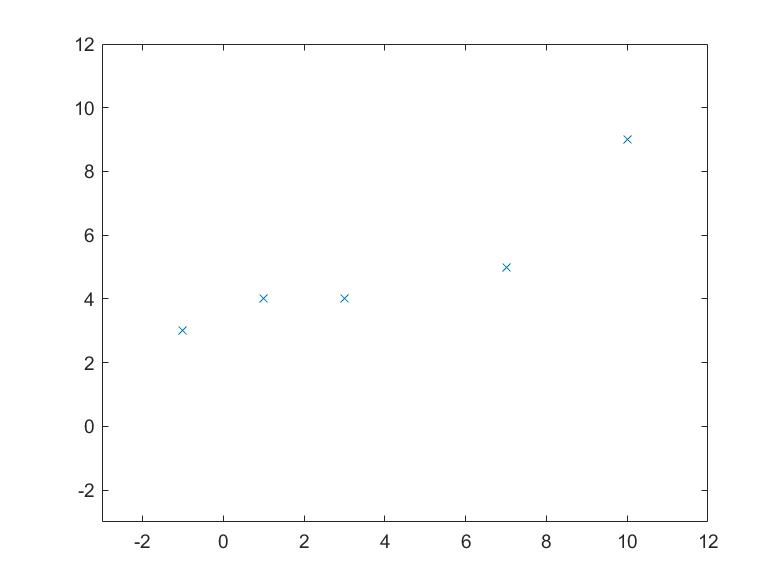
\includegraphics[scale=.3]{FacesNight7/figs/Dplot.jpg}
    \end{center}
    
    \item \begin{verbatim}
        >> mumatrix=[mean(D(:,1))*ones(5,1) mean(D(:,2))*ones(5,1)]
        >> tildeD=D-mumatrix
        >> plot(tildeD(:,1),tildeD(:,2),'x')
        >> axis ([-7 7 -7 7])
    \end{verbatim}
    \begin{center}
        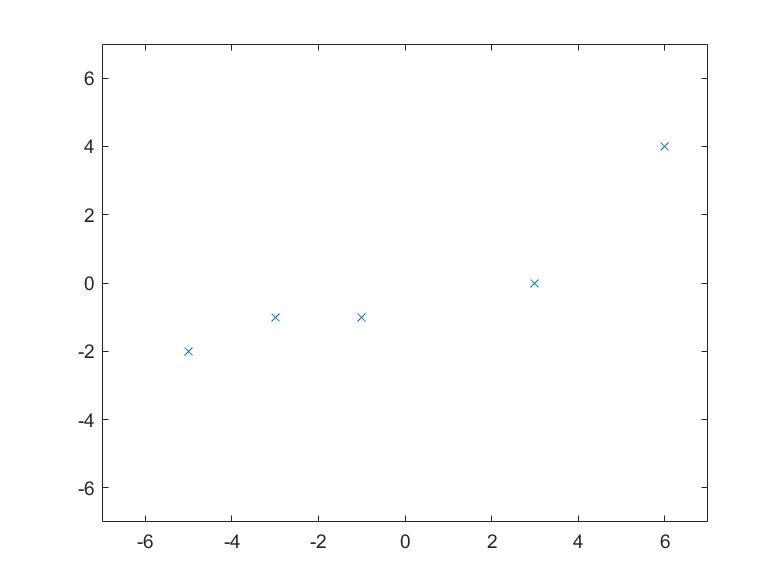
\includegraphics[scale=.3]{FacesNight7/figs/tildeDplot.jpg}
    \end{center}
    
    \item 
    \begin{verbatim}
    >> [Vec,Diam]=eig(tildeD'*tildeD)
    >> hold on
    >> quiver(0,0,Vec(1,1),Vec(2,1))
    >> quiver(0,0,Vec(1,2),Vec(2,2))
    \end{verbatim}
    \begin{center}
        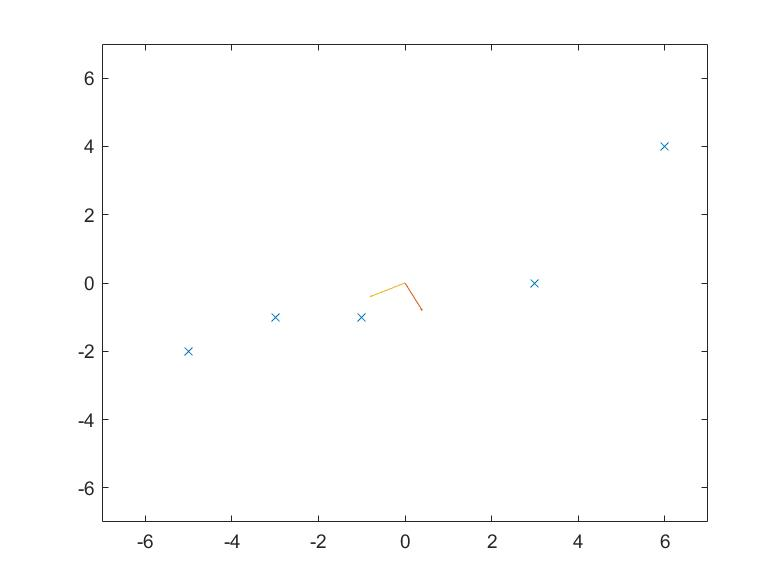
\includegraphics[scale=.3]{FacesNight7/figs/tildeDeigen.jpg}
    \end{center}
    
    \item
    \begin{verbatim}
    >> proj=tildeD*Vec(:,2)
    >> B=proj*Vec(:,2)'
    >> hold on
    >> plot(tildeD(:,1),tildeD(:,2),'x')
    >> plot(B(:,1),B(:,2),'o')
    >> axis ([-6 8 -6 8])
    \end{verbatim}
    \begin{center}
        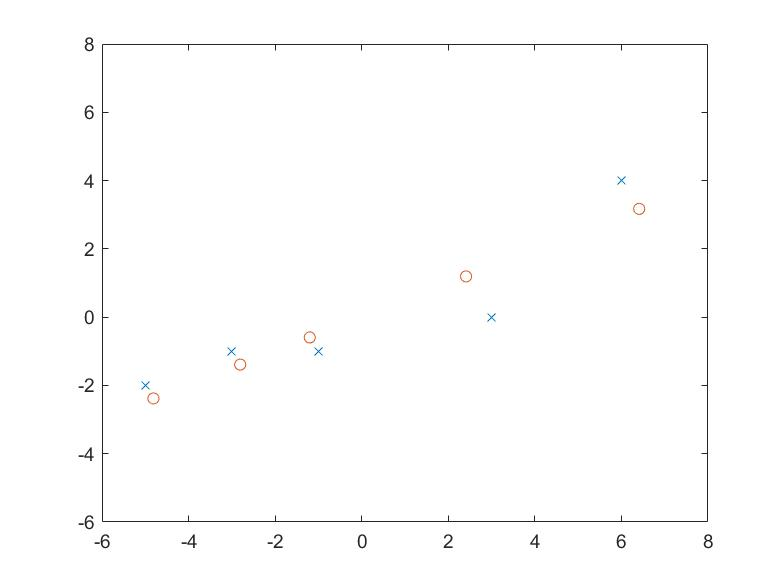
\includegraphics[scale=0.3]{FacesNight7/figs/reducedD.jpg}
    \end{center}
\end{enumerate}
\end{sol}

\begin{prob}
\begin{enumerate}
\item Can you recreate $\mathbf{D}$ perfectly from $\mathbf{B}$?
\item What would have happened if you had created $\mathbf{B}$ using only information about the values along $\mathbf{p_1}$ instead of $\mathbf{p_{2}}$?
\item How might you quantify how well you can represent $\mathbf{D}$ in this reduced dimensionality form?
\item If you received a new piece of data, how would you go about representing this as a linear combination of $\mathbf{p_{1}}$ and $\mathbf{p_2}$?
\end{enumerate}
\end{prob}
\begin{sol}
\begin{enumerate}
    \item No. If we write a data point $a\mathbf{p}_1 + b\mathbf{p}_2$, then the reduced dimension version is $b\mathbf{p}_2$. It's impossible to recover $a$, which is the information in the perpendicular direction.
    \item We would get the information in the perpendicular direction, which we can interpret as the ``error'' in reducing the dimension from $\mathbf{D}$ to $\mathbf{B}$.
    \item You can use the error $\mathbf{B}-\mathbf{D}$.
    \item We can write a new data point $\mathbf{d}$ as
    $$(\mathbf{d}\cdot\mathbf{p}_1)\mathbf{p}_1 + (\mathbf{d}\cdot\mathbf{p}_2)\mathbf{p}_2.$$
    \end{enumerate}
\end{sol}

\subsection{Data Compression via PCA}

In this exercise you will perform a simple data compression exercise, similar to the one you did in a previous Night assignment. You will use temperature data from 3 cities over 10 years, as training data and use it to compress a year's worth of temperature data from 3 cities into a $2\times 365$ matrix. In other words, you will represent $3\times 365$ numbers (daily temperature data from 3 cities over 1 year), using $2\times 365$ values. This compression is lossy, in that you will loose some information. However, by representing the data along the two most significant eigenvectors of the covariance matrix, you can reduce this data loss, because these two directions capture the bulk of the variation in the data set. Please note that while we have laid out the steps you need to take here quite explicitly, it is important for you to fully understand what each step does. You will be using very similar steps in your project.

\subsection{Exercises}
\begin{prob}
\begin{enumerate}
\item Load the file \texttt{avg\_temperatures\_pt2.mat}. You will have 6 data vectors in your workspace. \texttt{b\_tr, w\_tr, s\_tr}  which represent 10 years of training data for the average daily temperatures in Boston, Washington DC, and Sao Paolo, respectively. The vectors \texttt{b\_new, w\_new, s\_new} represent an additional year of data for the three cities -- this is the data that you will compress using statistical knowledge of the previous 10 years of data. Create a covariance matrix $\mathbf{R}$ using the 10 years worth of temperature data from Boston, Washington DC and Sao Paolo (in that order).

\item Perform an eigendecomposition of the matrix $\mathbf{R}$, and make a new matrix $\mathbf{V}_p$ which has the $2$ eigenvectors corresponding to the 2 largest eigenvalues of $\mathbf{R}$. You should use MATLAB's \texttt{eig} function. Let these eigenvectors be $\mathbf{v}_1$ and $\mathbf{v}_2$.

\item Create centered (i.e. subtract the mean), versions of the new temperature data vectors, and create a $3\times 365$ matrix $\mathbf{T}$ which has the centered temperatures of Boston, Washington DC and Sao Paolo as its rows (in that order). This matrix  is a representation of the data you are now going to compress. Let the $i$-th column of $\mathbf{T}$ be $\mathbf{t}_i$.

\item Take the dot product of each column of the matrix $\mathbf{T}$ (which is a vector of the temperature of Boston, Washington DC and Sao Paolo for a given day) with the two eigenvectors in matrix $\mathbf{V}_p$, and save the values.  Let this quantities be called $\alpha_{1i}$ and $\alpha_{2i}$. In other words,
    \begin{align*}
        \alpha_{1i} &= \mathbf{v}_1^T\mathbf{t}_i\\
        \alpha_{2i} &= \mathbf{v}_2^T\mathbf{t}_i
    \end{align*}
    You can do this using matrix multiplications.

    You should now have 365 different values for $\alpha_{1i}$ and $\alpha_{2i}$, which are a compressed representation of  $3\times 365$ different temperature values.  Moreover, these values are the components of the temperature data that lie in the directions of the two eigenvectors of the covariance matrix corresponding to the largest eigenvalues. From what we saw in the previous two classes, these vectors represent the two orthogonal directions in the data that have the most amount of variation, and hence the most "important" directions. Of course, there is a third direction (since the temperature vectors live in a 3-dimensional space), which we are discarding.  But since this is the direction  in which there is the least amount of variation in the data set, we do not lose too much information.

\item You can now check how well your compression worked, by using the values of $\alpha_{1i}$ and $\alpha_{2i}$ to reconstruct 365 different $3\times 1$ vectors each representing the temperatures for the three cities over the 365 days. Let $\hat{\mathbf{t}}_i$ represent the reconstructed temperature vector on the $i$-th day. Using what you know about  projections onto orthonormal vectors, reconstruct $\mathbf{t}_i$ using $\alpha_{1i}$, $\alpha_{2i}$, $\mathbf{v}_1$ and $\mathbf{v}_2$. Repeat this for all 365 days.

\item On the same axes, plot the original and reconstructed temperature for Boston. Repeat this for Washington DC and Sao Paolo. Observe how close the reconstructions are, for the different data sets.

\item How accurately do you think you can represent the data if you used 3 eigenvectors instead of 2?

\item If you feel inspired, repeat the above with temperature data for four different cities, and 2 or 3 different eigenvectors.

\end{enumerate}
\end{prob}
\begin{sol}
\begin{enumerate}
    \item \begin{verbatim}
>> A = (1/sqrt(7304))*[b_tr-mean(b_tr) w_tr-mean(w_tr) s_tr-mean(s_tr)];
>> R=A'*A
    \end{verbatim}
    \item \begin{verbatim}
>> [V,D]=eig(R)
>> Vp=[V(:,2) V(:,3)]
    \end{verbatim}
    \item \begin{verbatim}
>> T = [b_new-mean(b_new) w_new-mean(w_new) s_new-mean(s_new)]'
    \end{verbatim}
    \item \begin{verbatim}
>> alpha=Vp'*T;
    \end{verbatim}
\end{enumerate}
\end{sol}


While this example can be thought of as a ``toy'' example where we are representing 3 dimensional data using 2 dimensions, there are many applications for which there may be many more dimensions in the data for which accurate representations can be made using only a few dimensions. Additionally, you should note that such dimensionality reduction techniques are not just useful in compression, but they are also useful in speeding up computation. We can often get away with analyzing data over a small number of important dimensions, and this is an important technique when we deal with large amounts of data. Overall, these class of techniques is called Principal Component Analysis (PCA), since we are performing analysis along a few principal component directions of the data.

\section{Face Data Compression via PCA}

You are now ready to start applying PCA to face data.   You have already seen this in a previous class assignment, except in that assignment you had the help of a genie.  Load the MATLAB files \texttt{classdata\_train.mat} and \texttt{classdata\_test.mat}. These are the training and test datasets with photos of your classmates. The file contains some images and as well as the identity of the person in each image (coded as an integer from 1 to 89).%  I have also included the data file from last year in case you want more images.

Remember that the principal eigenvectors of the covariance matrix tell you the directions of greatest variation in a data set and also the directions that optimally compress our data.  Your job is to use the training images to build a model for your faces such that you can compress a many-pixeled test face image (pick one from the test image array) using a small set of image vectors (e.g., 10, 20, or 50).

Before you dig into this problem, think through how you would formalize the face data compression as a problem that you can solve with the linear algebra techniques that you've learned so far.  There is no exercise to answer, but we want you to think through these steps before going further in the assignment.

\begin{itemize}
\item How you will choose your set of image vectors?
\item Come up with the steps needed to do the above and write some pseudo code (e.g., load the data, vectorize the images, etc.).
\item How could you tell whether your compression algorithm works (these could either be quantitative metrics, like root-mean squared error or qualitative metrics).
\end{itemize}

\section{Eigenfaces for Face Recognition}

It's time to bring it all together and finally plunge into the prosopagnosia (look it up) problem (or at least build some facial recognition software, but alliteration is fun). You will implement the eigenfaces algorithm to identify photos of your classmates.  While it sounds fancy, you have almost all of the pieces needed to understand and implement Eigenfaces (the last necessary piece you will pick up momentarily).  Here are the major steps in the Eigenfaces algorithm.

\be
\item Use PCA to compute the $k$ principal components of the training face images (the $k$ eigenvectors with largest eigenvalues).
\item Project the training and test face images onto the $k$ principal components.  We'll call this the \emph{facespace} representation of our original images.
\item For each of the test images, compute the closest match between the test image (represented as a $k$-dimensional vector in facespace) and the training images (again, in facespace).  The notion of ``closest match'' here can be described in a few different ways, but the easiest thing to do is to use the the Euclidean distance to define how far apart two points are.  In this way, you would look for the training point that has the smallest Euclidean distance for a particular test point and predict the identity of the test point to be the same as the identity of this closest training point.  This method of classification is known as \href{https://en.wikipedia.org/wiki/K-nearest_neighbors_algorithm}{nearest neighbor classification} and it is the one new concept you need to implement Eigenfaces.
\ee


% As with any of these night assignments it is an individual assignment, so the material you turn in should be your own work, but you are welcome to discuss ideas with your classmates and teaching team.
%
%\begin{prob}
%Revisit and reflect on the concept map [2 hr]
%\begin{enumerate}
%\item Dig out your concept map from Day 1 (Canvas kindly saved this for you, as did your personal file organization system).
%\item Research eigenfaces and update your concept map
%\begin{itemize}
%\item Check out \href{https://drive.google.com/open?id=0B7LNBbaxYFujTkwxY1BZZEE2eWM}{an early paper on eigenfaces}. You have most of the tools to understand this paper, but the writing style might be unfamiliar (intense!). Spend 1-2 hours on this paper and then feel free to move on. The first 6 pages of this paper describe the use of eigenfaces in face recognition.
%    Check out other sources as well. Wikipedia is pretty useful for eigenfaces, and \href{https://drive.google.com/open?id=0B7LNBbaxYFujLUFfNThyT2JqNmc}{this} later paper talks about eigenfaces and an extension called Fisherfaces (not fish faces).
%\item While you are reading, highlight/color code your concept map to show two things:
%\begin{enumerate}
%\item concepts that are important in your readings about eigenfaces
%\item concepts that you understand or still need to spend some time learning (you choose which way to represent this)
%\end{enumerate}
%Make sure to indicate the legend of your color code. Feel free to update your concept map as needed. Turn this in.
%\end{itemize}
%\end{enumerate}
%\end{prob}

\begin{prob}
Earlier in this assignment you wrote some pseudo code for face compression, which as you can see from the description of Eigenfaces above, gets you most of the way there.  Before you actually implement Eigenfaces, we'd like you to extend your pseudocode to cover the whole Eigenfaces algorithm.  In addition to the steps of Eigenfaces describe above, you should also think about the steps needed to calculate the accuracy of your system (i.e., how often does it get the person's identity correct).
\end{prob}

\begin{prob}
Implement the eigenfaces algorithm.% from \href{https://drive.google.com/open?id=0B7LNBbaxYFujTkwxY1BZZEE2eWM}{this paper} in MATLAB. [5 hr]
\begin{enumerate}
\item Your code, which can be a script, function, or livescript, should use the training and test sets of images provided: \texttt{classdata\_train.mat} and \texttt{classdata\_test.mat}, respectively.
\item You may want to start by identifying one face from the test set, but by the time you are done, your code should run through all of the test images and report the fraction it guesses correctly.
\item Test different numbers of eigenvectors. How many does it take to guess right most of the time?
\item If you'd like, time how long it takes your code to run. Can you do anything more efficiently to make it run faster?   (use \texttt{tic} and \texttt{toc} in MATLAB for timing)
\item Visualize the first few eigenfaces.  Can you interpret what they mean?
\item Generate a figure that depicts the success rate (accuracy at determining the identify of a person in an image) versus the number of eigenfaces used.
\item Generate a figure that depicts the success rate (accuracy at determining the identify of a person in an image) versus the number of eigenfaces used where the training data consists of only images of people not smiling and the test data consists of only images of people smiling (these are located in \texttt{classdata\_non\_smiles.mat} and \texttt{classdata\_smiles.mat} respectively.  Comment on the difference in performance on when using these files versus the data from the previous parts of this problem.
\end{enumerate}

Guidelines:
\begin{itemize}
\item You should comment your code (use \texttt{\%}) so others could read and understand it.
\item Don't use the command \texttt{pca}, but instead build your algorithm using either the \texttt{eig} or \texttt{eigs} command (\texttt{eigs} computes just a few eigenvectors, which can be faster when you only care about the eigenvectors with large eigenvalues). We want you to think through all the steps involved in your facial recognition program, and that means doing the math ``yourself''.
\end{itemize}
\emph{(Optional)} Extensions (These are not spelled out in much detail.  We recommend you talk to a member of the teaching team before trying these (especially the second two).
\bi
\item Analyze the mistakes your algorithm makes (particularly when training on non-smiles and testing on smiles).
\item Use Eigenfaces to do smile detection instead of identity recognition.
\item Combine Eigenfaces with a classifier other than nearest neighbors (e.g., formulate an LSAE to create a series of one person versus everyone else detectors).
\item Get your system working on live video.
\ei
\end{prob}
\begin{sol}
A reference implementation of Eigenfaces is linked from the Canvas assignment page.
\end{sol}

\pagebreak
\shipoutAnswer

%
%\newpage
%
%\section{Derivations (optional reading!)}
%
%\subsection{Non-negativity of eigenvalues and orthogonality of eigenvectors of covariance matrices}
%
%Covariance matrices have non-negative eigenvalues, and their eigenvectors are mutually orthogonal.  These properties can be proved as follows. First let $\mathbf{A} = \mathbf{X}^T\mathbf{X}$, where $\mathbf{X}$ is our centralized data matrix (i.e. data matrix with the mean subtracted out). Let $\mathbf{v}_i$ and $\lambda_i$ be the $i$-th eigenvector and eigenvalue of $\A$ respectively.
%\[  \mathbf{X}^T\mathbf{X v}_i =\lambda_i \mathbf{v}_i \]
%Now we multiply both sides by $\v_i^T$
%\[ \mathbf{v}_i^T\mathbf{X}^T\mathbf{X v}_i =\lambda_i \mathbf{v}_i^T\mathbf{v}_i \]
%and use the properties of the transpose
%\[ (\mathbf{X}\mathbf{v}_i )^T\mathbf{X v}_i =\lambda_i \mathbf{v}_i^T\mathbf{v}_i \]
%and finally divide both sides by the scalar $\mathbf{v}_i^T\mathbf{v}_i$
%\[ \frac{(\mathbf{X}\mathbf{v}_i )^T\mathbf{X v}_i}{\mathbf{v}_i^T\mathbf{v}_i}=\lambda_i \]
%Both the numerator and denominator are the result of multiplying the transpose of a column vector with itself. Hence the numerator and denominator are non-negative, which yields the result that the eigenvalues are non-negative, i.e.
%\[ \lambda_i\geq 0 \]
%
%Next we shall show that the eigenvectors are orthogonal. Consider the case that $i\neq j$ and that the matrix $\mathbf{A}$ has distinct eigenvalues
%\[ \mathbf{Av}_i = \lambda_i \mathbf{v}_i \]
%Now we multiply both sides by $\v_j^T$
%\[ \mathbf{v}_j^T\mathbf{Av}_i = \lambda_i \mathbf{v}_j^T\mathbf{v}_i \]
%and use the properties of the transpose
%\[ (\mathbf{A}^T\mathbf{v}_j)^T\mathbf{v}_i = \lambda_i \mathbf{v}_j^T\mathbf{v}_i \]
%Since $\mathbf{A}$ is symmetric, we know that $\A^T = \A$ so that
%\[ (\mathbf{A}\mathbf{v}_j)^T\mathbf{v}_i = \lambda_i \mathbf{v}_j^T\mathbf{v}_i \]
%Recalling that $\v_j$ is an eigenvector of $\A$ with eigenvalue $\lambda_j$
%\[ (\lambda_j\mathbf{v}_j)^T\mathbf{v}_i = \lambda_i \mathbf{v}_j^T\mathbf{v}_i \]
%and using properties of the transpose
%\[ \lambda_j\mathbf{v}_j^T\mathbf{v}_i = \lambda_i \mathbf{v}_j^T\mathbf{v}_i \]
%Bringing everything to one side
%\[ \lambda_j\mathbf{v}_j^T\mathbf{v}_i - \lambda_i \mathbf{v}_j^T\mathbf{v}_i = 0 \]
%and factoring gives
%\[ (\lambda_j-\lambda_i)\mathbf{v}_j^T\mathbf{v}_i  = 0. \]
%Hence, if the eigenvalues are distinct, then it must be the case that $\mathbf{v}_j$ and $\mathbf{v}_i$ are orthogonal for $i\neq j$. Moreover, the eigenvectors can be made orthonormal by scaling each one.
%
%
%\subsection{Why does  the principal eigenvector of the covariance matrix point in the direction of greatest variation in the data?}
%Let $\mathbf{b}_i$ be defined as the vector made up of the $i$th data samples with the mean subtracted out. If for example, we are dealing with two data variables, $x$ and $y$ (e.g. representing temperature in Boston and Sao Paolo),
%\begin{align*}
%\mathbf{b}_i = \begin{pmatrix}
%x_i -\mu_x \\
%y_i -\mu_y
%\end{pmatrix}
%\end{align*}
%
%Now let's define a unit vector $\mathbf{u}$ which points in {\emph some} (at this point unknown) direction, with unit length. Recall from the take home exercise that the dot product of $\mathbf{u}$ and $\mathbf{b}_i$, tells you the length of the component of $\mathbf{b}_i$ that lies in the direction of $\mathbf{u}$. Let's define the length of this projection as $w_i$. Thus we have
%\begin{align}
%w_i = \mathbf{u} \cdot \mathbf{b}_i = \mathbf{u}^T \mathbf{b}_i
%\end{align}
%Hence,  $w_i$ is a measure of "how much" of $\mathbf{b}_i$ lies in the direction of $\mathbf{u}$.
%
%Recall that the variance of the set of data points $w_1, w_2, \cdots w_N$ is
%\begin{align}
%\sigma_w^2 = \frac{1}{N} \sum_{j = 1}^N (w_i - \mu_w)^2\,
%\end{align}
%where $\mu_w$ is the mean or average of $w_1, w_2, \cdots w_N$. Since $w_i$ measures the component of $\mathbf{b}_i$ that lies in the direction of $\mathbf{u}$, $\sigma^2_w$ is a measure of the variation in the data set in the direction of $\mathbf{u}$. The goal of the rest of this section is to prove that the $\mathbf{u}$ which maximizes $\sigma^2_w$ is precisely the principle eigenvector of the covariance matrix of the data.
%
%The mean of each entry in $\mathbf{b}_i$ is zero because $\mathbf{b}_i$ equals data samples with the means subtracted out, in other words, the entries of $\mathbf{b}_i$ have mean equal to zero. Hence,
%\begin{align*}
%\mu_w &= \frac{1}{N} \sum_{i = 1}^N w_i = \frac{1}{N} \sum_{i = 1}^N \mathbf{u}^T \mathbf{b}_i \\
%&=  \mathbf{u}^T \sum_{i = 1}^N \frac{1}{N} \mathbf{b}_i = \mathbf{0}\\
%\end{align*}
%
%
%Therefore we can rewrite $\sigma_w^2$ as
%\begin{align}
%\sigma_w^2 &= \frac{1}{N} \sum_{j = 1}^N w_i^2 = \frac{1}{N} \sum_{j = 1}^N (\mathbf{u}^T \mathbf{b}_i)^2 \\
%&= \sum_{j = 1}^N  \left(\frac{1}{\sqrt{N}}\mathbf{u}^T\mathbf{b}_i\right)\left(\frac{1}{\sqrt{N}}\mathbf{b}_i^T\mathbf{u}\right) \nonumber \\
%&= \frac1N\left[\mathbf{u}^T\mathbf{b}_1\; \mathbf{u}^T\mathbf{b}_2\; \cdots \; \mathbf{u}^T\mathbf{b}_N\right] \left[\mathbf{u}^T\mathbf{b}_1 \; \mathbf{u}^T\mathbf{b}_2 \; \cdots \; \mathbf{u}^T\mathbf{b}_N\right]^T \nonumber \\
%&= \frac1N\mathbf{u}^T\left[\mathbf{b}_1\; \mathbf{b}_2\; \cdots \; \mathbf{b}_N\right] \left[\mathbf{b}_1 \; \mathbf{b}_2 \; \cdots \; \mathbf{b}_N\right]^T \mathbf{u}
%\end{align}
%
%Define
%
%\begin{align*}
%\mathbf{A} = \frac{1}{\sqrt{N}} \begin{pmatrix}
%    {x_1-\mu_x} & {y_1-\mu_y}\\
%   {x_2-\mu_x} &  {y_2-\mu_y}\\
%    {x_3-\mu_x} & {y_3-\mu_y}\\
%    \vdots & \vdots \\
%    x_N - \mu_x & y_N - \mu_y
%  \end{pmatrix}
%\end{align*}
%and the covariance matrix of the data as $\mathbf{R} = \A^T\A$. From the definition of $\mathbf{b}_i$ and $\A$, we then have
%\begin{align}
%\sigma^2_w = \mathbf{u}^T \mathbf{A}^T\mathbf{A u} = \mathbf{u}^T\mathbf{Ru} \label{eqnQuadraticFormCov}
%\end{align}
%
%Since $\sigma_w^2$ is the variation in the data set in the direction $\mathbf{u}$, at this point, what is left is to show that the unit vector $\mathbf{u}$ which maximizes the above expression is precisely the principle eigenvector of the covariance matrix $\mathbf{R}$. Our strategy to do this is to find an upper bound to $\sigma_w^2$ and then show that the principle eigenvector results in a value of $\sigma_w^2$ which meets that upper bound.
%
%\subsection{An upper bound on the variation}
%To find the unit vector $\mathbf{u}$ which maximizes \eqref{eqnQuadraticFormCov} involves constrained optimization, since we are trying to maximize $\sigma_w^2$ subject to the constraint that $\mathbf{u}$ has unit length. Constrained optimization is a large, rich, and interesting topic. Fortunately (or unfortunately), we can do this particular constrained optimization using the tools we have already developed, without requiring a foray into advanced optimization techniques. To simplify matters, let's introduce a new vector $\mathbf{w}$ such that
%\begin{align}
%\mathbf{u} = \frac{\mathbf{w}}{||\mathbf{w}||} = \frac{\mathbf{w}}{\sqrt{\mathbf{w}^T\mathbf{w}}}
%\end{align}
%By this definition, $\mathbf{u}$ is a normalized version of $\mathbf{w}$, hence, $\mathbf{u}$ will have unit length, no matter what $\mathbf{w}$ is. Substituting this definition into \eqref{eqnQuadraticFormCov} yields
%
%\begin{align}
%\sigma^2_w = \frac{\mathbf{w}^T\mathbf{Rw}} {\mathbf{w}^T \mathbf{w}}  \label{eqnQuadraticFormCovConstrained}
%\end{align}
%Now, we need to maximize the above equation over any $\mathbf{w}$, which will result in a $\mathbf{u}$ which is automatically of unit length. Next, we perform an eigendecomposition on $\mathbf{R}$ as follows
%\begin{align*}
%\mathbf{R} = \mathbf{Q\Lambda Q}^{-1}\,.
%\end{align*}
%From what we know about the eigendecomposition, the columns of $\mathbf{Q}$ are the eigenvectors of $\mathbf{R}$ and $\mathbf{\Lambda}$ is a diagonal matrix containing the corresponding eigenvalues in its diagonal entries. Let these eigenvectors be denoted by $\mathbf{v}_1, \mathbf{v}_2$, and the corresponding eigenvalues be $\lambda_1, \lambda_2$. Here, we are assuming that we have two variables $x$ and $y$ in our data set, but these steps carry over directly to the case when we have more than two variables. We further know that the eigenvectors are orthongonal, because $\mathbf{R}$ is a covariance matrix. Additionally, we can normalize the eigenvectors to have unit length (in fact MATLAB's \texttt{eig} command produces normalized eigenvectors).
%
%Write the EVD of $\mathbf{R}$ as $\mathbf{R} = \mathbf{Q\Lambda Q}^T$. Hence, \eqref{eqnQuadraticFormCovConstrained} becomes
%
%\begin{align}
%\sigma^2_w &=  \frac{1}{\mathbf{w}^T \mathbf{w}}\mathbf{w}^T  \mathbf{Q\Lambda Q}^T \mathbf{w} \nonumber \\
% &=  \frac{1}{\mathbf{w}^T \mathbf{w}}\mathbf{w}^T \left[\mathbf{v}_1\; \mathbf{v}_2 \; \cdots \; \mathbf{v}_N \right] \Lambda \left[\mathbf{v}_1\; \mathbf{v}_2 \; \cdots \; \mathbf{v}_N \right]^T \mathbf{w}\nonumber  \\
% &=  \frac{1}{\mathbf{w}^T \mathbf{w}}\mathbf{w}^T \left[\lambda_1\mathbf{v}_1\; \lambda_2\mathbf{v}_2 \; \cdots \; \lambda_N\mathbf{v}_N \right] \left[\mathbf{v}_1\; \mathbf{v}_2 \; \cdots \; \mathbf{v}_N \right]^T \mathbf{w}\nonumber \\
%&=  \frac{1}{\mathbf{w}^T \mathbf{w}}\mathbf{w}^T \left[\lambda_1\mathbf{v}_1\; \lambda_2\mathbf{v}_2 \; \cdots \; \lambda_N\mathbf{v}_N \right] \left( \mathbf{w}^T\left[\mathbf{v}_1\; \mathbf{v}_2 \; \cdots \; \mathbf{v}_N \right]\right)^T\nonumber \\
%&=  \frac{1}{\mathbf{w}^T \mathbf{w}} \left[\lambda_1\mathbf{w}^T\mathbf{v}_1\; \lambda_2\mathbf{w}^T\mathbf{v}_2 \; \cdots \; \lambda_N\mathbf{w}^T\mathbf{v}_N \right]  \left[\mathbf{w}^T\mathbf{v}_1\; \mathbf{w}^T\mathbf{v}_2 \; \cdots \; \mathbf{w}^T\mathbf{v}_N \right]^T \nonumber \\
%&= \frac{1}{\mathbf{w}^T \mathbf{w}}\sum_{i = 1}^2 \mathbf{w}^T  \mathbf{v}_i \lambda_i \mathbf{w}^T\mathbf{v}_i  = \frac{\sum_{i = 1}^2 \mathbf{w}^T  \mathbf{v}_i \lambda_i \mathbf{v}_i^T \mathbf{w}}{\mathbf{w}^T \mathbf{w}} \nonumber \\
%& = \frac{1}{\mathbf{w}^T \mathbf{w}}\sum_{i = 1}^2 \lambda_i \mathbf{w}^T  \mathbf{v}_i  \mathbf{v}_i^T \mathbf{w}\label{eqnVariationInterm}
%\end{align}
%
%
%Since the eigenvectors $\mathbf{v}_i$ form a basis in $\R^2$ (for the case of 2 variables), and $\mathbf{w}^T\mathbf{v}_i$ is the projection of $\mathbf{w}$ onto $\mathbf{v}_i$ we can write the following
%\begin{align}
%\mathbf{w} = \sum_{i = 1}^2\alpha_i\mathbf{v}_i. \label{eqnEVecdecomp}
%\end{align}
%where $\alpha_i = \mathbf{w}^T\mathbf{v}_i$.
%Using this property, we have that
%
%\begin{align*}
%\mathbf{w}^T \mathbf{w} &= \left(\sum_{i = 1}^2\alpha_i\mathbf{v}_i\right)^T \left(\sum_{j = 1}^2\alpha_i\mathbf{v}_j\right) \\
%&= (\alpha_1\mathbf{v}_1 +\alpha_2\mathbf{v}_2)^T (\alpha_1\mathbf{v}_1 +\alpha_2\mathbf{v}_2)\\
%&=(\alpha_1\mathbf{v}_1^T +\alpha_2\mathbf{v}_2^T)(\alpha_1\mathbf{v}_1 +\alpha_2\mathbf{v}_2)\\
%&=\alpha_1^2\mathbf{v}_1^T\mathbf{v}_1  +  \alpha_1\alpha_2\mathbf{v}_1^T\mathbf{v}_2  + \alpha_2\alpha_1\mathbf{v}_2^T\mathbf{v}_1  + \alpha_2^2\mathbf{v}_2^T\mathbf{v}_2
%\end{align*}
%
%Since $\v_1$ and $\v_2$ are orthonormal, $\v_1^T\v_1 = 1, \v_2^T\v_2 = 1$ and $\v_1^T\v_2 = 0$. Therefore, the sum above only has two non-zero terms,
%\begin{align*}
%\mathbf{w}^T \mathbf{w} &= \alpha_1^2\mathbf{v}_1^T\mathbf{v}_1   + \alpha_2^2\mathbf{v}_2^T\mathbf{v}_2 = \alpha_1^2 + \alpha_2^2 \label{eqnWNormSq}
%\end{align*}
%
%
%Substituting  $\alpha_i = \mathbf{w}^T\mathbf{v}_i$ into the numerator and \eqref{eqnWNormSq} into the deniminator of  \eqref{eqnVariationInterm} yields
%\begin{align}
%\sigma^2_w  &= \frac{\sum_{i = 1}^2 \lambda_i \alpha_i^2  }{\sum_{j = 1}^2 \alpha_j^2}
%\end{align}
%
%Now let $\lambda_M$ denote the largest eigenvalue. Hence, we have
%
%\begin{align}
%\sigma^2_w &= \frac{\sum_{i = 1}^2 \lambda_i \alpha_i^2 }{\sum_{j = 1}^2 \alpha_j^2}\nonumber \\
%& \leq  \frac{\sum_{i = 1}^2 \lambda_M \alpha_i^2 }{\sum_{j = 1}^2 \alpha_j^2} = \lambda_M  \label{eqnQuadFormUB}
%\end{align}
%
%The bound above tells us that the maximum variation in the data along any direction $\mathbf{u}$ is at most $\lambda_M$. Next, we shall show that if $\mathbf{u}$ is the eigenvector corresponding to the largest eigenvalue of $\mathbf{R}$, i.e. the principal eigenvector, then the bound above is met.
%Let $\mathbf{v}_M$ denote the eigenvector corresponding to the largest eigenvalue of $\mathbf{R}$, and let $\mathbf{u} = \v_M$.  Substitute this into
%\eqref{eqnQuadraticFormCov} yields
%\begin{align}
%\sigma_w^2 = \v_M^T\mathbf{R}\v_M
%\end{align}
%
%Performing an EVD on $\mathbf{R}$ again yields
%\begin{align}
%\sigma_w^2 &= \v_M^T\mathbf{QRQ}^T\v_M\\
%&= \v_M^T \left[\mathbf{v}_1\; \mathbf{v}_2 \; \cdots \; \mathbf{v}_N \right] \Lambda \left[\mathbf{v}_1\; \mathbf{v}_2 \; \cdots \; \mathbf{v}_N \right]^T\v_M\\
% &=\left[\v_M^T\mathbf{v}_1\; \v_M^T\mathbf{v}_2 \; \cdots \; \v_M^T\mathbf{v}_N \right] \begin{bmatrix}\lambda_1 & & \\ & \ddots &\\ & & \lambda_N \end{bmatrix} \left[\v_M^T\mathbf{v}_1\; \mathbf{v}_2 \; \cdots \; \mathbf{v}_N \right]^T
%\end{align}
%Since $\mathbf{v}_M\mathbf{v}_i$ is non-zero except for $i = M$, the only non-zero entry in $\left[\v_M^T\mathbf{v}_1\; \v_M^T\mathbf{v}_2 \; \cdots \; \v_M^T\mathbf{v}_N \right]$ is equal to 1 and in the position that $v_M$ is located in. Hence, the above expression simplifies to
%
%\begin{align}
%\sigma_w^2 &= \v_M^T\v_M\lambda_M \v_M^T\v_M = \lambda_M
%\end{align}
%Since $\sigma_w^2$ is the variance of the data that is projected onto the vector $\mathbf{u} = \mathbf{v}_M$, and this variance equals the upper bound on the variance, we conclude that the variance is maximized along the direction of $\v_M$, which is the eigenvector corresponding to the largest eigenvalue of the covariance matrix $\mathbf{R}$.
%
%The above example was for $2$ dimensional covariance matrices, but the ideas extend to higher dimensions as well, whereby the eigenvector corresponding to the largest eigenvalue points in the direction of greatest variance, and the eigenvector corresponding to the second largest eigenvalue points in the direction that has the most variation in the data, which is orthogonal to the direction of the principal eigenvector, and so on.
%
%
%
%\subsection{Why does SVD work?}
%
%Let's consider the product $\A^T \A$: all non-zero eigenvalues of this matrix are positive. If $\lambda_i$ is a non-zero eigenvalue of $\A^T \A$ with eigenvector $\v_i$, then we can write
%\[\A^T \A \v_i = \sigma_i^2 \v_i \]
%where $\sigma_i = \sqrt{\lambda_i}$. If we left multiply by $\v_i^T$ we get
%\[ \v_i^T \A^T \A \v_i = \v_i^T \sigma_i^2 \v_i \]
%and if we use the fact that $\v_i$ is normalized and the properties of transposes
%\[(\A \v_i)^T (\A \v_i) = \sigma_i^2 \]
%which shows that the length of the vector $\A \v_i$ is just $\sigma_i$.
%
%Let's return to our earlier statement
%\[ \A^T \A \v_i = \sigma_i^2 \v_i \]
%Now if we left multiply by $\A$ we get
%\[ \A \A^T \A \v_i = \sigma_i^2 \A \v_i \]
%and so $\A \v_i$ is an eigenvector of $\A \A^T$ with eigenvalue $\sigma_i^2$. So $\u_i = \A \v_i / \sigma_i$ is a unit eigenvector of $\A \A^T$ and we have
%\[ \A \v_i = \sigma_i \u_i \]
%This allows us to write
%\[ \A \onebythree{\v_1}{\ldots}{\v_r} = \onebythree{\u_1}{\ldots}{\u_r} \threebythree{\sigma_1}{}{}{}{\cdot}{}{}{}{\sigma_r} \]
%Since the columns of $\mathbf{V}$ are orthonormal we can right multiply by $\mathbf{V}^T$ to get
%\[ \A = \onebythree{\u_1}{\ldots}{\u_r} \threebythree{\sigma_1}{}{}{}{\cdot}{}{}{}{\sigma_r}  \onebythree{\v_1}{\ldots}{\v_r}^T \]
%or simply
%\[ \A = \mathbf{U} \mathbf{\Sigma} \mathbf{V}^T \]
%which is just the SVD of $\A$.